% Provenance (never printed): old terminale S material on past climates (ice cores,
% pollen, ocean sediments and oxygen isotopes, glacial-interglacial cycles, the
% astronomical rhythm told, climates of deep time), read from data. Owner (Sync 0/1):
% climate archive and proxy, ice core, glacial period, interglacial and glacial cycle,
% pollen analysis, Last Glacial Maximum. Recalled: glacier, ice sheet, ice age (Book 1,
% grade 8); the first look at the ice-core records (Book 1, grade 9); isotopes
% (physics); greenhouse gases (chemistry); the time scale (Book 1, grade 7). The
% delta notation of isotopes is Book 3's: isotope curves are read here as told,
% without a definition. The orbital theory of climate belongs to a university book:
% told here only. Physical science only, in the IPCC's calibrated words.
% Figures: figdata/grade-12/ice_age_records.py (tests/grade-12/test_ice_age_records.py).
\chapter{Reading Past Climates}\label{ch:g12:past-climates}

At Dome~C, \qty{3233}{m} high on the East Antarctic ice sheet, the air
averages about \qty{-55}{\degreeCelsius} over the year. A drill working there
stopped at a depth of \qty{3260}{m}, about \qty{15}{m} above the rock beneath
the ice. The deepest ice it brought up holds tiny bubbles of air some
\num{800000} years old: a sample of the atmosphere from long before the
first farmers. This chapter
reads the climate of the past in the ice, in the mud of lakes and of the
ocean floor, and in the rocks, and asks what it says about today.
% ledger: ipev:concordia, edc3:drilling, jouzel07:edc

\begin{omfigure}
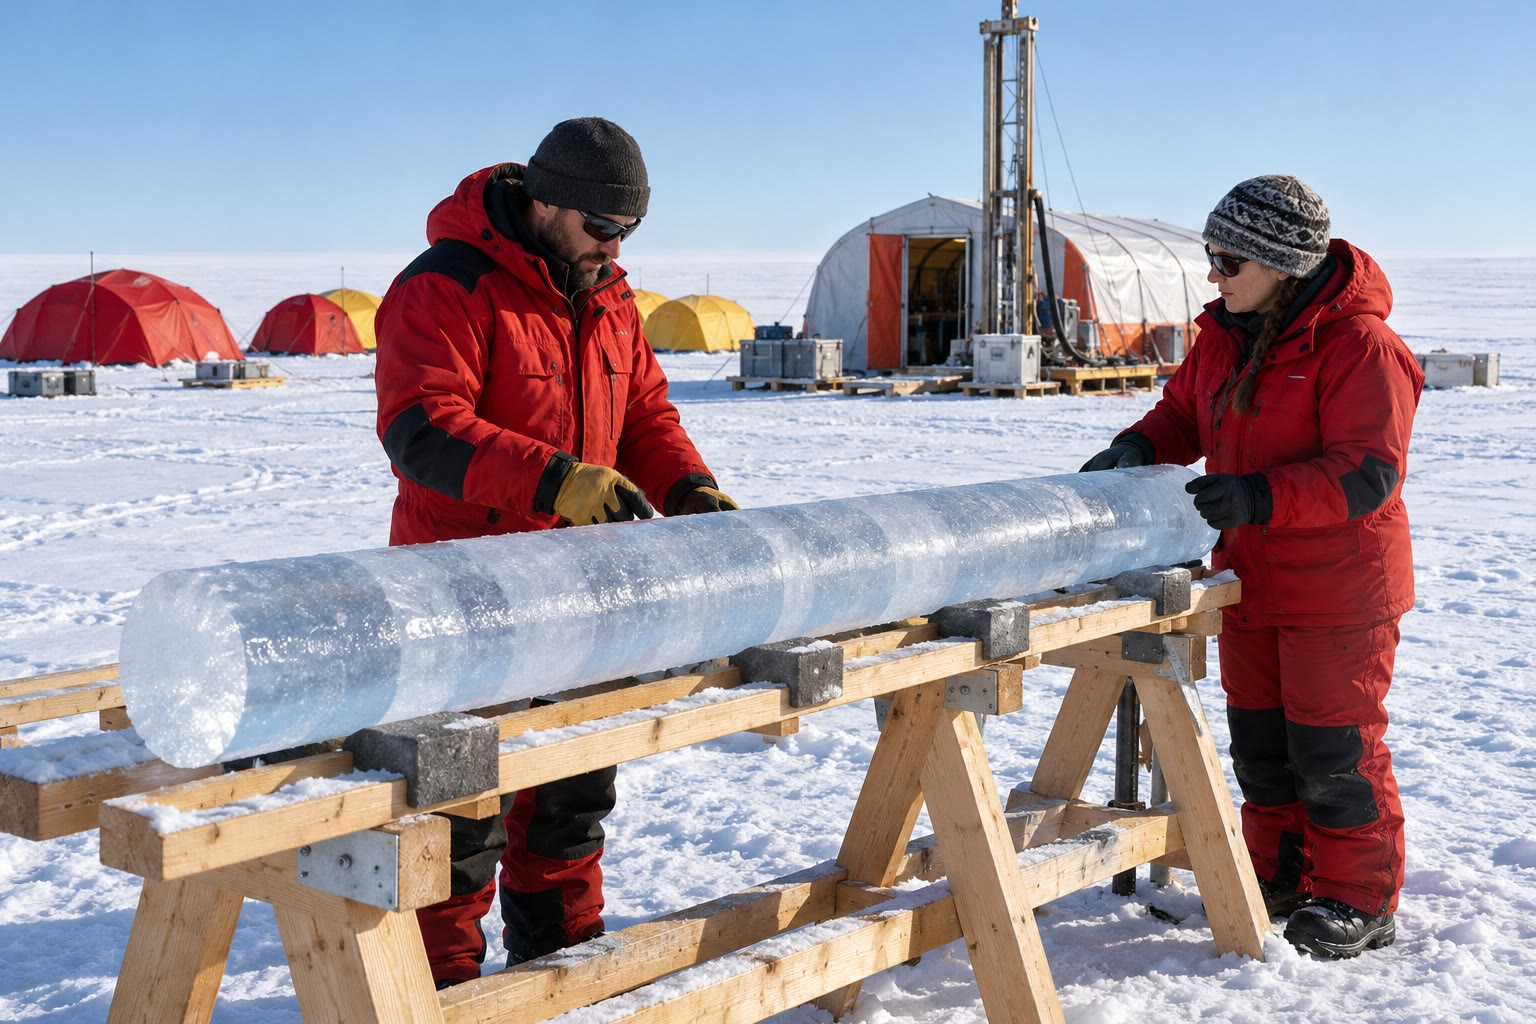
\includegraphics[width=0.56\linewidth]{images/book2/ai/g12-ice-coring-camp.jpg}

{\small An ice-coring camp on a polar ice sheet: the drill works under the
tower and the shelter, and each length of core is laid out, logged and
packed before it travels to the laboratory. AI-generated illustration.}
\end{omfigure}

\begin{recall}
A glacier is a mass of ice that lasts from year to year and flows under its
own weight; an ice sheet covers a large part of a continent; an ice age is a
long cold time when ice sheets spread far beyond the poles (Book 1, grade 8).
In the \omterm{def:g12:past-climates:ice-core}{ice cores} of Antarctica, the snow records the air temperature and the
bubbles keep the air itself, and the two records rise and fall together
(Book 1, grade 9). Atoms of one element may differ by their number of
neutrons: these isotopes behave alike in chemistry but differ in mass (the
physics books). Carbon dioxide is a greenhouse gas (the chemistry books).
The Quaternary period began 2.58 million years ago
(Book 1, grade 7).
\end{recall}
% ledger: ics:base.Quaternary (shared), nasaeo:o18 (snow poor in heavy isotopes)

\section{Archives and proxies}

Nobody measured the temperature of the air \num{20000} years ago. But the
Earth kept records without meaning to: layers of ice and mud, shells and tree
trunks, each of which changed with the climate in which it formed.

\begin{definition}[Climate archive; proxy]\label{def:g12:past-climates:proxy}
A \emph{climate archive}\index{climate archive} is a natural material laid
down in layers, one after another, that keeps a trace of the climate of the
time it formed: polar ice, the sediments of lakes and of the ocean floor, the
rings of trees, corals, cave deposits. A \emph{proxy}\index{proxy} is a
quantity measured in an archive that stands in for a climate variable that
was not measured: the share of heavy isotopes in old snow for the air
temperature, the share of each kind of pollen in lake mud for the vegetation
and so for the climate.
\end{definition}
% ledger: ncei:proxy, ncei:pollen, nasaeo:o18

\begin{center}
\small
\begin{tabular}{|l|l|l|}
\hline
\textbf{archive} & \textbf{\omterm{def:g12:past-climates:proxy}{proxy}} & \textbf{tells about} \\
\hline
polar ice & heavy isotopes of the ice & air temperature over the ice \\
 & air in the bubbles & carbon dioxide, methane \\
lake sediments, peat & pollen & vegetation, then climate \\
ocean sediments & oxygen isotopes of shells & ice volume, deep-water temperature \\
tree rings & ring width & growing conditions, year by year \\
corals, cave deposits & isotopes, growth bands & sea or air temperature, rain \\
\hline
\end{tabular}

\medskip
{\small The main \omterm{def:g12:past-climates:proxy}{climate archives} and some of their proxies.}
\end{center}
% ledger: ncei:proxy, nasaeo:o18

Every \omterm{def:g12:past-climates:proxy}{proxy} needs two things before it can be read. It needs a \emph{clock}:
the age of each layer, from counting yearly layers where they can be seen,
from radiometric dating (\cref{ch:g12:age-of-the-earth}), or from matching the
record with another one already dated. And it needs a \emph{calibration}: the
link between what is measured and the climate variable, found today, where
both can be measured together.

\begin{method}[Reading a proxy record]
\begin{enumerate}
  \item Find the archive and the \omterm{def:g12:past-climates:proxy}{proxy}: what was measured, and in what?
  \item Find which way time runs on the axis, and in what unit; check
        whether the \omterm{def:g12:past-climates:proxy}{proxy} axis is reversed.
  \item Translate the \omterm{def:g12:past-climates:proxy}{proxy}: does a higher value mean warmer or colder,
        more ice or less?
  \item Note the spacing of the samples: a record whose points are
        \num{2000} years apart cannot show a change that lasted a century.
  \item Read the values at the dates asked, or the means over an interval,
        and compute changes and rates.
  \item Say what the record shows at its site, and only then whether it
        speaks for the whole Earth.
\end{enumerate}
\end{method}

\section{Ice cores}

\begin{definition}[Ice core]\label{def:g12:past-climates:ice-core}
An \emph{ice core}\index{ice core} is a cylinder of ice drilled out of an ice
sheet or a glacier. Its depth gives the age of the ice, the deeper the older;
the ice records the temperature of the air in which its snow fell, and its
bubbles keep samples of the air of the time.
\end{definition}
% ledger: ncei:proxy, jouzel07:edc

Fresh snow is mostly air. Buried under the snow of the following years, it is
pressed into \emph{firn}, a compacted snow whose pores still let air through.
At a density of about 820 to \qty{830}{kg/m^3}, reached 50 to \qty{120}{m}
down, the pores close and the air is sealed in bubbles. The ice therefore keeps two different
records. The air in the bubbles is a sample of the atmosphere, whose carbon
dioxide and methane are measured in the laboratory. The ice itself holds the
temperature: water molecules that contain a heavy isotope (deuterium or
oxygen-18) condense more readily than the light ones, so the colder the air
on the way to the pole, the poorer the snow becomes in heavy isotopes.
% ledger: firn:close-off, nasaeo:o18

\begin{omfigure}
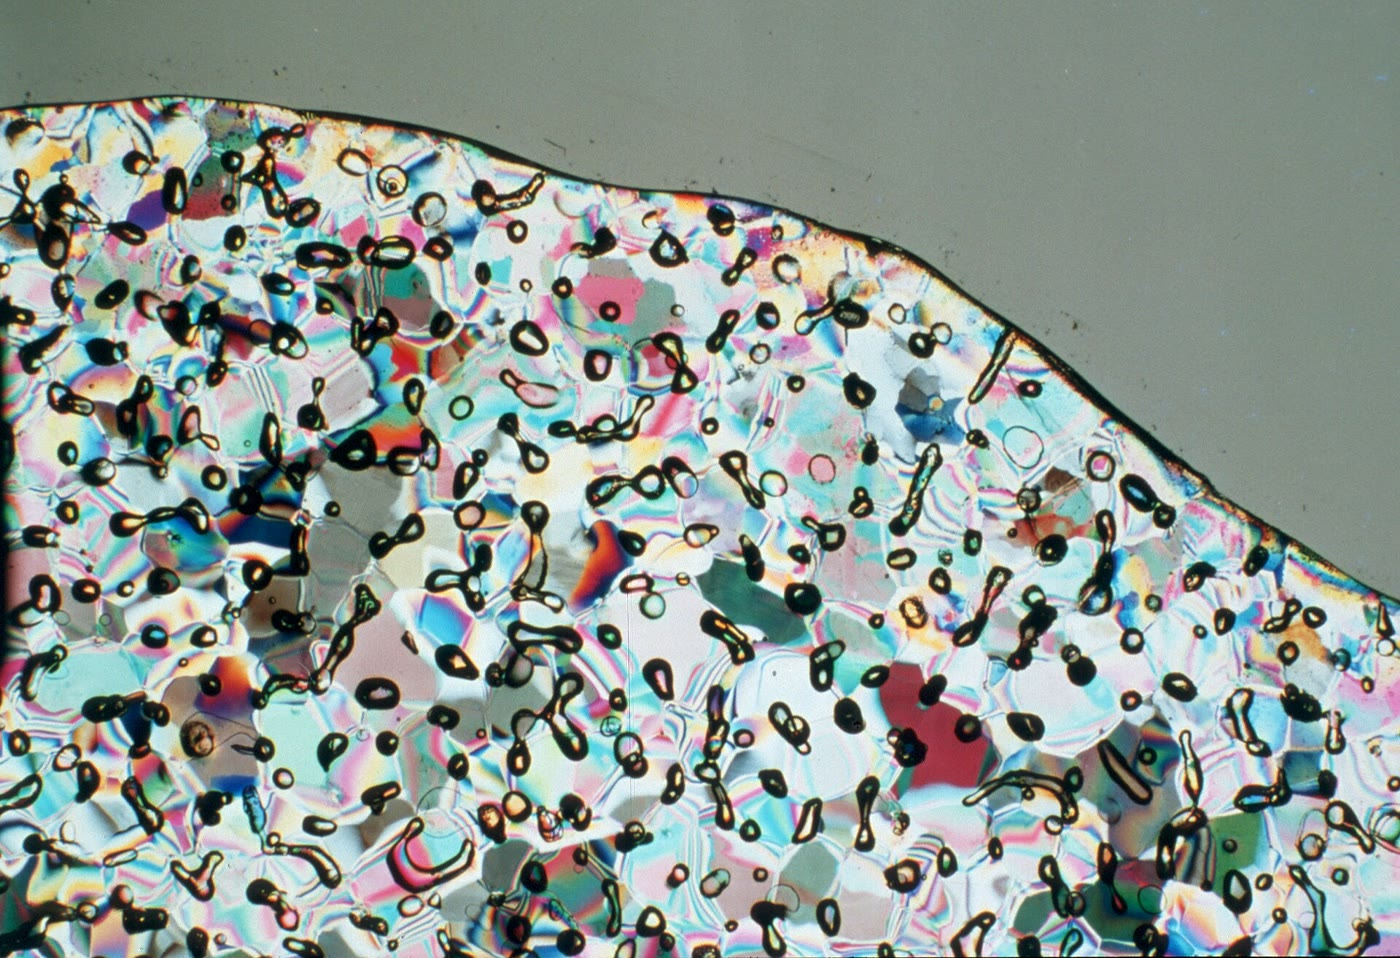
\includegraphics[width=0.50\linewidth]{images/book2/g12-ice-bubbles.jpg}

{\small A sliver of Antarctic ice seen under polarised light, which colours
the ice crystals: the dark dots are bubbles of trapped air. Photograph CSIRO
Atmospheric Research, CC~BY~3.0 (Wikimedia Commons).}
\end{omfigure}
% ledger: photo:g12-ice-bubbles

The deuterium of the Dome~C core has been turned into a temperature over the
ice, given as a change compared with the mean of the last thousand years. The
carbon dioxide comes from the bubbles of several Antarctic cores, put
together into one record. Both are drawn below on one time axis.

\begin{omfigure}
\begin{tikzpicture}
\begin{axis}[omrecord, scale only axis, width=0.74\linewidth, height=4.8cm,
  xmin=0, xmax=800, x dir=reverse, ymin=-12, ymax=8, axis y line*=left,
  xtick={0,100,...,800}, ytick={-10,-5,0,5},
  xlabel={thousands of years before 1950},
  ylabel={temperature change (\unit{\degreeCelsius})}]
% data:edc-jouzel, 2-kyr means (figdata/grade-12/ice_age_records.py)
\addplot[omWarm, line width=0.7pt] table[x=age_kyr, y=temp_C] {figdata/out/grade-12-ice_age_records-edc.dat};
\end{axis}
\begin{axis}[scale only axis, width=0.74\linewidth, height=4.8cm,
  xmin=0, xmax=800, x dir=reverse, ymin=60, ymax=320, axis y line*=right,
  axis x line=none, ytick={180,220,260,300}, ylabel={carbon dioxide (ppm)},
  every axis label/.append style={font=\small}, tick label style={font=\small}]
% data:co2-bereiter, 2-kyr means
\addplot[black, line width=0.7pt] table[x=age_kyr, y=co2_ppm] {figdata/out/grade-12-ice_age_records-co2.dat};
\coordinate (lt) at (axis cs:560,70);
\coordinate (lc) at (axis cs:560,312);
\end{axis}
\node[font=\scriptsize, text=omWarm, anchor=south] at (lt) {temperature at Dome~C (left scale)};
\node[font=\scriptsize, anchor=north] at (lc) {carbon dioxide (right scale)};
\end{tikzpicture}

{\small Eight hundred thousand years of Antarctic ice, averaged over steps of
\num{2000} years. Red: the temperature at Dome~C compared with the last
thousand years (Jouzel and others, 2007); black: the carbon dioxide of the
bubbles (Bereiter and others, 2015). Today is on the right.}
\end{omfigure}
% ledger: data:edc-jouzel, data:co2-bereiter

The two curves share one pattern: a slow, ragged slide into the cold over
tens of thousands of years, then a fast climb back to warmth, then the
slide again.

\begin{definition}[Glacial period; interglacial; glacial cycle]\label{def:g12:past-climates:glacial-cycle}
A \emph{glacial period}\index{glacial period} is a cold interval within an
ice age, during which the ice sheets grow far beyond their present size. An
\emph{interglacial}\index{interglacial} is a warm interval between two
glacial periods, with ice sheets close to today's or smaller; we live in one,
which began about \num{11000} years ago. A \emph{glacial
cycle}\index{glacial cycle} is one glacial period with the interglacial that
ends it.
\end{definition}
% ledger: ipcc:ref-periods (LDT ends 11 ka); the count of cycles is read from the figure (data:edc-jouzel)

Over the whole record, the temperature at Dome~C ranges from
\qty{-10.6}{\degreeCelsius}, about \num{24000} years ago, to
\qty{+5.5}{\degreeCelsius}, about \num{129000} years ago; the carbon dioxide,
from \qty{174}{ppm} to \qty{299}{ppm}. The figure, averaged over \num{2000}
years, smooths these extremes a little. A count of the warm peaks gives eight
or nine \omterm{def:g12:past-climates:glacial-cycle}{glacial cycles}, and the strongest rhythm of the temperature record,
computed from its data, has a period of about \num{98000} years.
% ledger: data:edc-jouzel, data:co2-bereiter (ice_age_records.py: edc_min_C -10.58 at 24.0 kyr, edc_max_C 5.46 at 128.7 kyr, co2 173.71 and 298.6, edc_period_kyr 97.5)

\begin{proposition}[Temperature and carbon dioxide vary together]\label{prop:g12:past-climates:correlation}
% ledger: data:edc-jouzel, data:co2-bereiter (ice_age_records.py: r_temp_co2 0.9165, fit 266.57 + 7.827 T, 1639 pairs)
Over the last \num{800000} years, the Antarctic temperature and the carbon
dioxide of the air varied together. Pairing each of the 1639 carbon dioxide
measurements older than \num{2000} years with the Dome~C temperature at the
same age gives a correlation coefficient of $r = 0.92$, and the
least-squares line
\[
  \mathrm{CO_2} \approx \qty{267}{ppm} + \qty{7.8}{ppm/\degreeCelsius} \times \Delta T ,
\]
where $\Delta T$ is the temperature change at Dome~C.
\end{proposition}

\begin{proof}[How it is computed]
For each carbon dioxide sample, the temperature at its age is read in the
Dome~C record by interpolating between the two nearest temperature points.
The correlation coefficient of the 1639 pairs, a number between $-1$ and $1$
that measures how close the points lie to a straight line (the mathematics
books), is computed with the least-squares line; both are computed in the
figure script and checked by its test.
\end{proof}

\begin{omfigure}
\begin{tikzpicture}
\begin{axis}[omrecord, width=0.70\linewidth, height=5.2cm, xmin=-12, xmax=6,
  ymin=160, ymax=310, xlabel={temperature change at Dome~C (\unit{\degreeCelsius})},
  ylabel={carbon dioxide (ppm)}]
% data:edc-jouzel, data:co2-bereiter (pairs and fit in ice_age_records.py)
\addplot[only marks, mark=*, mark size=0.6pt, omDef, opacity=0.45] table[x=temp_C, y=co2_ppm] {figdata/out/grade-12-ice_age_records-pairs.dat};
\addplot[omThm, line width=1pt] table[x=temp_C, y=co2_ppm] {figdata/out/grade-12-ice_age_records-fit.dat};
\node[font=\scriptsize, text=omThm, anchor=south east, fill=white, inner sep=1pt] at (axis cs:-1.5,295) {least-squares line, $r = 0.92$};
\end{axis}
\end{tikzpicture}

{\small Each dot is one carbon dioxide measurement of the Antarctic ice,
placed at the Dome~C temperature of the same age: cold ages had little carbon
dioxide, warm ages much more. Computed from Jouzel and others (2007) and
Bereiter and others (2015).}
\end{omfigure}

A correlation does not say which changed first, nor whether a third cause
moved both: the coefficient would be the same if temperature drove carbon
dioxide, if carbon dioxide drove temperature, or if each pushed the other.
What sets the rhythm of about \num{100000} years is told in the section on
the ocean below, and how carbon dioxide acts on temperature in
\cref{ch:g12:climate-change}.

\subsection{The Last Glacial Maximum}

\begin{definition}[Last Glacial Maximum]\label{def:g12:past-climates:lgm}
The \emph{Last Glacial Maximum}\index{Last Glacial Maximum} is the time, about
\num{23000} to \num{19000} years ago, when the ice sheets of the last \omterm{def:g12:past-climates:glacial-cycle}{glacial
period} were at their largest.
\end{definition}
% ledger: ipcc:ref-periods

At the \omterm{def:g12:past-climates:lgm}{Last Glacial Maximum}, ice sheets covered much of North America and of
north-western Eurasia, and the climate was drier and dustier than today. The
assessments estimate that the global surface temperature was \qty{5}{\degreeCelsius}
to \qty{7}{\degreeCelsius} lower than in 1850--1900 (\emph{medium confidence}),
with the carbon dioxide at 188 to \qty{194}{ppm}. The water locked in the ice
sheets came from the ocean: global mean sea level stood 125 to \qty{134}{m}
below today's.
% ledger: ipcc:ref-periods, ipcc:lgm-cooling, ipcc:fig2-34, ipcc:lgm-sea, lambeck14:lgm

A lower sea uncovers the shallow floor around the continents. The map below
lowers the sea by \qty{130}{m}, the middle of that range, over the floor of
South-East Asia as it is today.

\begin{omfigure}
\begin{tikzpicture}
\begin{axis}[omrecord, axis equal image, width=0.62\linewidth, xmin=92, xmax=122,
  ymin=-11, ymax=24, grid=none, axis x line=box, axis y line=box,
  xtick={95,105,115}, ytick={-10,-5,...,20},
  xticklabel={\pgfmathprintnumber{\tick}\textdegree E},
  yticklabels={10\textdegree S, 5\textdegree S, 0\textdegree, 5\textdegree N, 10\textdegree N, 15\textdegree N, 20\textdegree N}]
% data:b2-etopo-sunda (raster computed in ice_age_records.py; sea level lowered by 130 m)
\addplot graphics[xmin=91.95, xmax=122.05, ymin=-11.05, ymax=24.05] {figdata/out/grade-12-ice_age_records-sunda.png};
\node[font=\scriptsize] at (axis cs:114.5,0.5) {Borneo};
\node[font=\scriptsize, rotate=-45] at (axis cs:101.9,-1.3) {Sumatra};
\node[font=\scriptsize] at (axis cs:110.5,-8.6) {Java};
\node[font=\scriptsize, rotate=-60] at (axis cs:102.2,4.0) {Malay Pen.};
\node[font=\scriptsize] at (axis cs:103,16.5) {Indochina};
\node[font=\scriptsize, align=center] at (axis cs:106.5,3.5) {Sunda\\Shelf};
\node[font=\scriptsize, align=center] at (axis cs:114.5,13) {South China\\Sea};
\node[font=\scriptsize, align=center] at (axis cs:96,-6) {Indian\\Ocean};
\end{axis}
\end{tikzpicture}

{\small South-East Asia with the sea \qty{130}{m} lower than today. Green:
land today; tan: the floor that a sea level \qty{130}{m} lower uncovers; blue:
sea. The present relief is used, so the coastline is only approximate.
Computed from the ETOPO1 relief (NOAA), every 0.1 degree.}
\end{omfigure}
% ledger: data:b2-etopo-sunda, ipcc:lgm-sea

Borneo, Sumatra and Java become one land with the Malay Peninsula and
Indochina: the Sunda Shelf, under a shallow sea today, was dry land. On the map, a
fall of only about \qty{36}{m} is enough to join Borneo to Asia, and Sumatra and
Java join it sooner. On the map,
the land above the sea grows from 4.11 to 7.16 million square kilometres,
1.74 times as much. Over the whole Earth, the same \qty{130}{m} fall raises
the share of the surface above the sea from \qty{29.0}{\percent} to
\qty{33.5}{\percent}, about 23 million square kilometres of new land.
% ledger: data:b2-etopo-sunda, data:etopo1 (ice_age_records.py: borneo_link_m -36; sunda_land_now_km2 4.105e6, lgm 7.161e6, ratio 1.744; world_land_now_frac 0.2904, lgm 0.3352, world_gain_km2 2.285e7)

\begin{example}[The last deglaciation]
The warming that followed the \omterm{def:g12:past-climates:lgm}{Last Glacial Maximum} is called the last
deglacial transition; the assessments place it between about \num{18000} and
\num{11000} years ago. In the Dome~C record, the mean temperature of the
\omterm{def:g12:past-climates:lgm}{Last Glacial Maximum} (\num{23000} to \num{19000} years ago) is
\qty{-9.4}{\degreeCelsius}; the mean of the following interval \num{11000} to
\num{9000} years ago is \qty{-0.4}{\degreeCelsius}. The air over Antarctica
warmed by \qty{9.0}{\degreeCelsius}, while its carbon dioxide rose from
\qty{190}{ppm} to \qty{264}{ppm}, by \qty{74}{ppm}. Over the whole Earth,
the warming was the assessed cooling of 5 to \qty{7}{\degreeCelsius}, about
\qty{6}{\degreeCelsius}, spread over the \num{7000} years of the transition:
\[
  \frac{\qty{6}{\degreeCelsius}}{\num{7000}\ \text{years}} \approx
  \qty{0.86}{\degreeCelsius} \text{ per thousand years.}
\]
Sea level rose meanwhile from about \qty{-120}{m} to \qty{-50}{m}, about
\qty{10}{mm} a year on average.
\end{example}
% ledger: ipcc:ref-periods, ipcc:lgm-cooling, ipcc:lgm-sea, data:edc-jouzel, data:co2-bereiter (ice_age_records.py: edc_lgm_C -9.389, edc_holo_C -0.360, rise 9.029; co2 189.67, 264.10, rise 74.43; ldt_mean_rate 0.857)

\begin{omfigure}
\begin{tikzpicture}
\begin{axis}[omrecord, scale only axis, width=0.74\linewidth, height=4.6cm,
  xmin=0, xmax=30, x dir=reverse, ymin=-11, ymax=12, axis y line*=left,
  xtick={0,5,...,30}, ytick={-10,-5,0},
  xlabel={thousands of years before 1950},
  ylabel={temperature change (\unit{\degreeCelsius})}]
\fill[omDef!10] (axis cs:23,-11) rectangle (axis cs:19,12);
\fill[omProp!12] (axis cs:18,-11) rectangle (axis cs:11,12);
% data:edc-jouzel, every sample
\addplot[omWarm, line width=0.6pt] table[x=age_kyr, y=temp_C] {figdata/out/grade-12-ice_age_records-edc30.dat};
\coordinate (lgm) at (axis cs:21,11.6);
\coordinate (ldt) at (axis cs:14.5,11.6);
\coordinate (lt) at (axis cs:5.5,-3.6);
\end{axis}
\begin{axis}[scale only axis, width=0.74\linewidth, height=4.6cm,
  xmin=0, xmax=30, x dir=reverse, ymin=60, ymax=290, axis y line*=right,
  axis x line=none, ytick={200,240,280}, ylabel={carbon dioxide (ppm)},
  every axis label/.append style={font=\small}, tick label style={font=\small}]
% data:co2-bereiter, every sample
\addplot[black, line width=0.6pt, mark=*, mark size=0.5pt] table[x=age_kyr, y=co2_ppm] {figdata/out/grade-12-ice_age_records-co230.dat};
\coordinate (lc) at (axis cs:26.5,196);
\end{axis}
\node[font=\scriptsize, anchor=north, align=center] at (lgm) {Last Glacial\\Maximum};
\node[font=\scriptsize, anchor=north, align=center] at (ldt) {last deglacial\\transition};
\node[font=\scriptsize, text=omWarm, anchor=north] at (lt) {temperature (left)};
\node[font=\scriptsize, anchor=south] at (lc) {carbon dioxide (right)};
\end{tikzpicture}

{\small The last \num{30000} years at Dome~C, every measurement: the
temperature (red) and the carbon dioxide (black) climb together out of the
\omterm{def:g12:past-climates:lgm}{Last Glacial Maximum}. Shaded: the \omterm{def:g12:past-climates:lgm}{Last Glacial Maximum} and the last deglacial
transition as dated by the IPCC. Data: Jouzel and others (2007), Bereiter and
others (2015).}
\end{omfigure}
% ledger: data:edc-jouzel, data:co2-bereiter, ipcc:ref-periods

\section{Pollen}

Every spring, plants release clouds of pollen. Most of it is lost, but some
falls on lakes and bogs, sinks, and is buried in the mud, where it keeps a
record of the vegetation that grew around. And the grains of each kind of
plant have their own shape and size.
% ledger: ncei:pollen

\begin{omfigure}
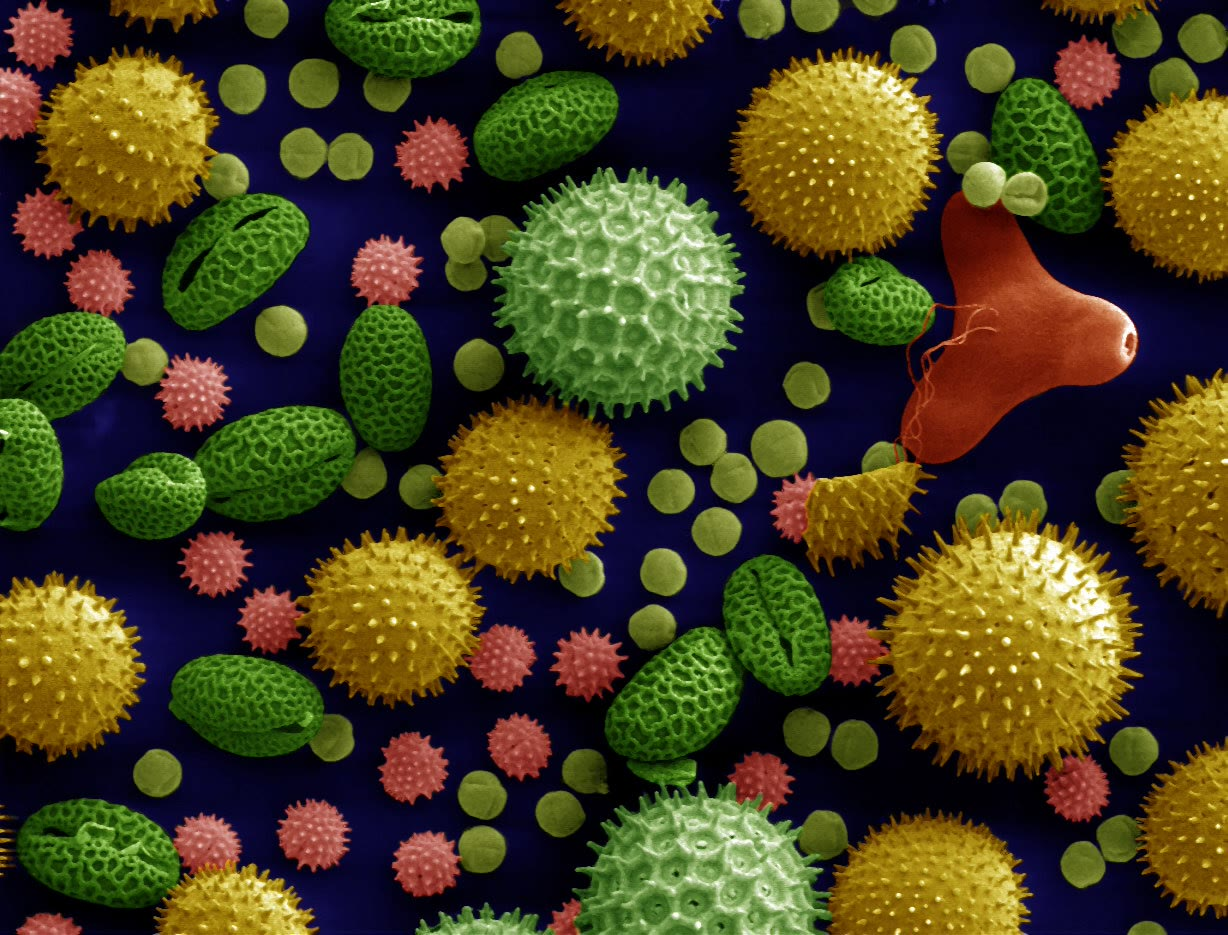
\includegraphics[width=0.46\linewidth]{images/book2/g12-pollen-sem.jpg}

{\small Pollen grains of five common plants (sunflower, morning glory,
hollyhock, lily and primrose) seen with a scanning electron microscope, in
false colours. Each kind of plant has its own shape of grain. Dartmouth
Electron Microscope Facility (public domain, via Wikimedia Commons).}
\end{omfigure}
% ledger: photo:g12-pollen

\begin{definition}[Pollen analysis]\label{def:g12:past-climates:pollen}
\emph{Pollen analysis}\index{pollen analysis} is the reading of past
vegetation from the pollen preserved in sediments: in each layer of a core,
the grains are identified and counted, and the share of each kind of plant,
in per cent of the grains counted, is plotted against depth in a
\emph{pollen diagram}\index{pollen diagram}.
\end{definition}
% ledger: ncei:pollen

Counting pollen in this way began with the Swedish geologist Lennart von
Post, who presented the first modern \omterm{def:g12:past-climates:pollen}{pollen diagram}, with numbers, in 1916;
such a diagram shows depth down the page and one curve for each kind of
plant. The vegetation, in its turn, speaks of the climate: grasses and other
herbs with almost no trees mean an open, cold landscape, while oak and
hazel need warm summers.
% ledger: rull18:von-post; the Varden diagram is invented (ice_age_records.py POLLEN)

\begin{omfigure}
\begin{tikzpicture}
\pgfplotsset{pollen/.style={scale only axis, height=6cm, ymin=300, ymax=600,
  y dir=reverse, xmin=0, axis x line*=bottom, axis y line*=left, axis line style={-},
  tick label style={font=\scriptsize}, title style={font=\small, yshift=-4pt, text depth=0.25ex, text height=1.6ex},
  ytick={300,350,...,600}, xmajorgrids, ymajorgrids,
  grid style={gray!22, line width=0.3pt}}}
\begin{axis}[pollen, name=p1, width=3.0cm, xmax=100, xtick={0,20,...,80}, title={herbs},
  ylabel={depth (cm)}, every axis label/.append style={font=\small}]
\addplot[fill=omLithSand, draw=black!70, line width=0.4pt] table[x=pct, y=depth_cm] {figdata/out/grade-12-ice_age_records-pol-herbs.dat};
\coordinate (z1) at (axis cs:0,550);
\coordinate (z2) at (axis cs:0,470);
\coordinate (z3) at (axis cs:0,425);
\end{axis}
\begin{axis}[pollen, name=p2, at={(p1.south east)}, anchor=south west, xshift=0.3cm,
  width=1.8cm, xmax=60, xtick={0,20,40}, title={birch}, yticklabels={}]
\addplot[fill=omHypsLandB, draw=black!70, line width=0.4pt] table[x=pct, y=depth_cm] {figdata/out/grade-12-ice_age_records-pol-birch.dat};
\end{axis}
\begin{axis}[pollen, name=p3, at={(p2.south east)}, anchor=south west, xshift=0.3cm,
  width=1.8cm, xmax=60, xtick={0,20,40}, title={pine}, yticklabels={}]
\addplot[fill=omHypsLandA, draw=black!70, line width=0.4pt] table[x=pct, y=depth_cm] {figdata/out/grade-12-ice_age_records-pol-pine.dat};
\end{axis}
\begin{axis}[pollen, name=p4, at={(p3.south east)}, anchor=south west, xshift=0.3cm,
  width=1.2cm, xmax=40, xtick={0,20}, title={hazel}, yticklabels={}]
\addplot[fill=omHypsLandD, draw=black!70, line width=0.4pt] table[x=pct, y=depth_cm] {figdata/out/grade-12-ice_age_records-pol-hazel.dat};
\end{axis}
\begin{axis}[pollen, name=p5, at={(p4.south east)}, anchor=south west, xshift=0.3cm,
  width=1.5cm, xmax=50, xtick={0,20,40}, title={oak}, yticklabels={}]
\addplot[fill=omHypsLandE, draw=black!70, line width=0.4pt] table[x=pct, y=depth_cm] {figdata/out/grade-12-ice_age_records-pol-oak.dat};
\coordinate (e1) at (axis cs:50,550);
\coordinate (e2) at (axis cs:50,470);
\coordinate (e3) at (axis cs:50,425);
\coordinate (top) at (axis cs:50,300);
\coordinate (bot) at (axis cs:50,600);
\end{axis}
\draw[densely dashed, black!70] (z1) -- (e1 -| p5.east);
\draw[densely dashed, black!70] (z2) -- (e2 -| p5.east);
\draw[densely dashed, black!70] (z3) -- (e3 -| p5.east);
\node[font=\scriptsize, anchor=west] at ($(bot -| p5.east)!0.5!(e1 -| p5.east)$) {zone 1};
\node[font=\scriptsize, anchor=west] at ($(e1 -| p5.east)!0.5!(e2 -| p5.east)$) {zone 2};
\node[font=\scriptsize, anchor=west] at ($(e2 -| p5.east)!0.5!(e3 -| p5.east)$) {zone 3};
\node[font=\scriptsize, anchor=west] at ($(e3 -| p5.east)!0.5!(top -| p5.east)$) {zone 4};
\node[font=\scriptsize, anchor=north] at ($(p1.south)!0.5!(p5.south)+(0,-0.45)$) {per cent of the pollen counted};
\end{tikzpicture}

{\small A \omterm{def:g12:past-climates:pollen}{pollen diagram} of a lake in the Varden Hills, the invented region
of this series: invented exercise data, with the succession found in many
lakes of the cool temperate zone. The bottom of the core (\qty{600}{cm}) is
\num{14000} years old, the top shown (\qty{300}{cm}) \num{6000} years old,
with a steady rate of deposition between.}
\end{omfigure}
% invented exercise data (ice_age_records.py POLLEN); no ledger row

\begin{method}[Reading a pollen diagram]
\begin{enumerate}
  \item Read the vertical axis: depth, the oldest layers at the bottom;
        turn depths into ages with the dates of the core.
  \item For each layer, find the plants with the largest shares.
  \item Divide the core into zones, each with its own set of dominant
        plants; place the limits where the curves change fastest.
  \item Name the vegetation of each zone (open herbs, birch woodland, pine
        forest, broadleaf forest) and the climate it needs.
  \item Read the zones from the bottom up as a history of the landscape.
\end{enumerate}
\end{method}

In the diagram above, zone 1 is a landscape of herbs, with a few birches: the
open, cold country left by the ice. In zone 2, birch spreads first, a hardy
tree; pine follows in zone 3; and in zone 4 hazel and oak, which need warm
summers, take over. Read from the bottom up, the core tells the end of the
\omterm{def:g12:past-climates:glacial-cycle}{glacial period} and the arrival of the warmth of the \omterm{def:g12:past-climates:glacial-cycle}{interglacial}, as the
forest moved back into the land.

\section{Ocean sediments and the astronomical rhythm}

On the floor of the open ocean, mud piles up slowly and without a break,
layer upon layer, for millions of years. It is full of the shells of
foraminifera: single-celled organisms whose shell, a fraction of a
millimetre across, is often made of calcite. Some float near the
surface; others live on the sea floor.
% ledger: ucmp:forams, lr04:stack (benthic), photo:g12-forams (planktic)

\begin{omfigure}
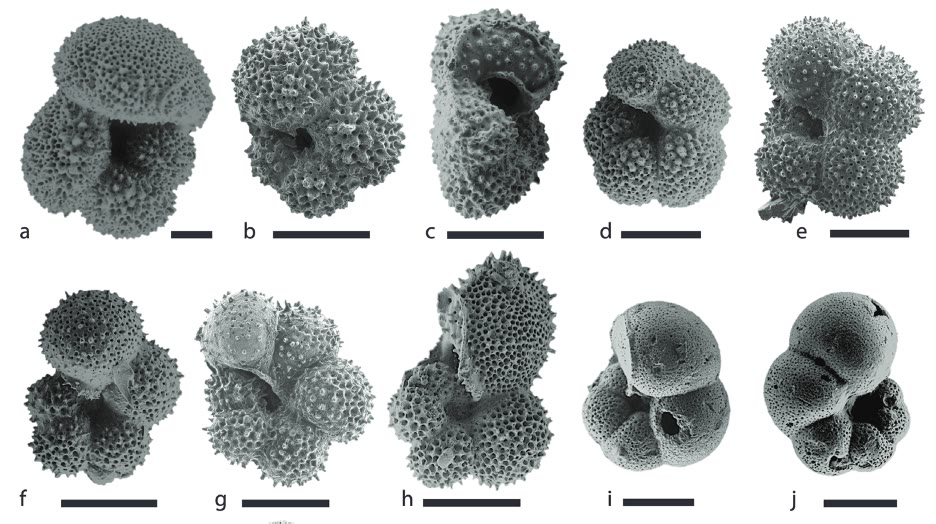
\includegraphics[width=0.62\linewidth]{images/book2/g12-planktic-foraminifera.jpg}

{\small Shells of ten species of foraminifera that lived floating in the
ocean, seen with a scanning electron microscope; each scale bar is
\qty{150}{\micro\metre}, so each shell is about the size of a grain of sand.
Marci Robinson, USGS (public domain, via Wikimedia Commons).}
\end{omfigure}
% ledger: photo:g12-forams

The oxygen of a shell comes from the sea water. Water made with the light
isotope oxygen-16 evaporates more easily, and the snow that builds the ice
sheets is therefore poor in oxygen-18. When the ice sheets grow, they store
this light water, and the ocean left behind becomes richer in oxygen-18; so
do the shells that grow in it, all the more as the water is colder. The share
of oxygen-18 in the shells of the sea-floor foraminifera, written
$\delta^{18}\mathrm{O}$ and given in parts per thousand, is thus a \omterm{def:g12:past-climates:proxy}{proxy} for
the volume of ice on land and for the temperature of the \omterm{def:g10:layered-ocean:thermocline}{deep ocean}: the
higher it is, the more ice and the colder the water.
% ledger: nasaeo:o18, lr04:stack

The record below, called LR04, stacks the measurements of 57 cores from all
the oceans into one curve of 5.3 million years.

\begin{omfigure}
\begin{tikzpicture}
\begin{axis}[omrecord, scale only axis, width=0.86\linewidth, height=4.8cm,
  xmin=0, xmax=5.32, x dir=reverse, ymin=2.4, ymax=5.3, y dir=reverse,
  xtick={0,0.5,...,5}, ytick={2.5,3,...,5},
  x tick label style={/pgf/number format/.cd, fixed, precision=1},
  y tick label style={/pgf/number format/.cd, fixed, fixed zerofill, precision=1},
  xlabel={millions of years before 1950},
  ylabel={$\delta^{18}\mathrm{O}$ of the shells (\unit{\permil})}]
\fill[omProp!14] (axis cs:1.25,2.4) rectangle (axis cs:0.7,5.3);
% data:lr04 (the stack only; ice_age_records.py)
\addplot[omDef!85!black, line width=0.35pt] table[x=age_Ma, y=d18O] {figdata/out/grade-12-ice_age_records-lr04.dat};
\addplot[omThm, line width=1pt, densely dashed, unbounded coords=jump] table[x=age_Ma, y=d18O] {figdata/out/grade-12-ice_age_records-lr04mean.dat};
\coordinate (mpt) at (axis cs:0.975,2.45);
\coordinate (mm) at (axis cs:5.22,4.92);
\coordinate (arr) at (axis cs:5.12,3.9);
\end{axis}
\node[font=\scriptsize, anchor=north, align=center] at (mpt) {41 000 to\\100 000 years};
\draw[omThm, line width=1pt, densely dashed] (mm) -- ($(mm)+(0.5,0)$) node[right, font=\scriptsize, text=omThm] {means of 5.3 to 3 and of 1 to 0 million years ago};
\draw[-{Stealth}, black!70] (arr) -- ++(0,-0.9) node[midway, right, font=\scriptsize, align=left] {more ice,\\colder};
\end{tikzpicture}

{\small Five million years of the \omterm{def:g10:layered-ocean:thermocline}{deep ocean} in the shells of sea-floor
foraminifera; the vertical axis is reversed, so that cold, icy times are
low. The dashed lines are the means of the first and last parts. Shaded:
the change from a rhythm of \num{41000} years to one of about \num{100000}
years. Data: Lisiecki and Raymo (2005), the LR04 stack.}
\end{omfigure}
% ledger: data:lr04, lr04:stack, clark06:mpt

Read with the method above, the record says three things.
\begin{itemize}
  \item \emph{The Earth has cooled and its ice has grown.} The mean value
        rises from \qty{3.03}{\permil} between 5.3 and 3 million years
        ago to \qty{4.15}{\permil} over the last million years.
  \item \emph{The swings have grown.} Glacial and \omterm{def:g12:past-climates:glacial-cycle}{interglacial} times
        alternate all along the record, but they swing wider and wider: at
        the \omterm{def:g12:past-climates:lgm}{Last Glacial Maximum} the value was \qty{4.92}{\permil}, against
        \qty{3.23}{\permil} today.
  \item \emph{The rhythm has changed.} Between 2.6 and 1.3 million years
        ago, the strongest period of the record, computed from its data, is
        \num{41000} years; over the last \num{700000} years it is about
        \num{98000} years, the rhythm of the \omterm{def:g12:past-climates:ice-core}{ice cores}. The change took
        place between about 1.25 and 0.7 million years ago.
\end{itemize}
% ledger: data:lr04, clark06:mpt (ice_age_records.py: lr04_mean_3_5Ma 3.032, lr04_mean_0_1Ma 4.147, lr04_lgm 4.92, lr04_today 3.23, periods 41.0 and 98.5 kyr)

These periods are not chance. In 1976, James Hays, John Imbrie and Nicholas
Shackleton found in the sediments of the southern oceans three rhythms, of
\num{23000}, \num{42000} and about \num{100000} years, which are the periods
of slow changes in the Earth's orbit and axis: the precession of the axis,
the tilt of the axis (about \num{41000} years) and the shape of the orbit
(about \num{100000} years). These changes move the sunlight that each
latitude receives in each season, and they set the pace of the \omterm{def:g12:past-climates:glacial-cycle}{glacial
cycles}. How they do so, and why the slow \num{100000}-year rhythm took
over, is the subject of a university course.
% ledger: hays76:periods, nasa:milankovitch, lr04:stack, clark06:mpt

\begin{dated}{2025}
In January 2025, the Beyond EPICA project announced that a core drilled at
Little Dome~C, about \qty{35}{km} from the Concordia station on Dome~C, holds
a continuous record back to about 1.2 million years in its upper
\qty{2480}{m}. It covers the time
when the glacial rhythm changed from \num{41000} to \num{100000} years, and the
ice and its air are being analysed.
\end{dated}
% ledger: ku25:beyond-epica, ipev25:little-dome-c

\section{Climates of deep time}

Further back than the \omterm{def:g12:past-climates:ice-core}{ice cores}, the climates of the past are read from
sediments, fossil leaves and soils, and isotopes. The IPCC has picked a few
\emph{reference periods}, well studied, whose climates help to judge
the changes of today and tomorrow. The chart below gives their global
surface temperature, compared with 1850--1900.

\begin{omfigure}
\begin{tikzpicture}
\begin{axis}[omrecord, width=0.86\linewidth, height=5.4cm, xmin=-9, xmax=27,
  ymin=0.4, ymax=6.6, y dir=reverse, ytick={1,...,6}, ymajorgrids=false,
  yticklabels={{PETM, 56 Ma}, {EECO, 53--49 Ma}, {MPWP, 3.3--3.0 Ma},
    {LIG, 129--116 ka}, {LGM, 23--19 ka}, {MH, 6.5--5.5 ka}},
  y tick label style={font=\scriptsize},
  xlabel={temperature compared with 1850--1900 (\unit{\degreeCelsius})}]
% ipcc:fig2-34 (DEEP in ice_age_records.py)
\addplot[draw=none, mark=none, restrict expr to domain={\thisrow{tlo}}{0:30},
  error bars/.cd, x dir=both, x explicit,
  error bar style={line width=5pt, omWarm!75}, error mark=none]
  table[x expr={(\thisrow{tlo}+\thisrow{thi})/2}, y=idx,
        x error expr={(\thisrow{thi}-\thisrow{tlo})/2}] {figdata/out/grade-12-ice_age_records-deep.dat};
\addplot[draw=none, mark=none, restrict expr to domain={\thisrow{tlo}}{-30:-0.01},
  error bars/.cd, x dir=both, x explicit,
  error bar style={line width=5pt, omCold!75}, error mark=none]
  table[x expr={(\thisrow{tlo}+\thisrow{thi})/2}, y=idx,
        x error expr={(\thisrow{thi}-\thisrow{tlo})/2}] {figdata/out/grade-12-ice_age_records-deep.dat};
\draw[black!60] (axis cs:0,0.4) -- (axis cs:0,6.6);
\draw[omThm, densely dashed, line width=0.8pt] (axis cs:1.09,0.4) -- (axis cs:1.09,6.6);
\node[font=\scriptsize, text=omThm, anchor=west, fill=white, inner sep=1pt] at (axis cs:1.6,4.55) {2011--2020};
\end{axis}
\end{tikzpicture}

{\small Global surface temperature of six reference periods of the past,
very likely ranges, compared with 1850--1900; dashed: the decade 2011--2020.
PETM: Paleocene--Eocene Thermal Maximum; EECO: Early Eocene Climatic
Optimum; MPWP: mid-Pliocene Warm Period; LIG: Last Interglacial; LGM: \omterm{def:g12:past-climates:lgm}{Last
Glacial Maximum}, the only cold one (blue); MH:
mid-Holocene. Values: IPCC AR6 WG1, Figure 2.34.}
\end{omfigure}
% ledger: ipcc:fig2-34, ipcc:gsat-2011-2020, ipcc:ref-periods

\begin{center}
\small
\begin{tabular}{|l|c|c|c|}
\hline
\textbf{period} & \textbf{temperature (\unit{\degreeCelsius})} & \textbf{carbon dioxide (ppm)} & \textbf{sea level (m)} \\
\hline
PETM, 56 Ma & $+10$ to $+25$ & about 900, rising to 2000 & --- \\
EECO, 53--49 Ma & $+10$ to $+18$ & 1150 to 2500 & $+70$ to $+76$ \\
MPWP, 3.3--3.0 Ma & $+2.5$ to $+4.0$ & 360 to 420 & $+5$ to $+25$ \\
LIG, 129--116 ka & $+0.5$ to $+1.5$ & 266 to 282 & $+5$ to $+10$ \\
\textcolor{omCold}{LGM, 23--19 ka} & \textcolor{omCold}{$-7$ to $-5$} & \textcolor{omCold}{188 to 194} & \textcolor{omCold}{$-134$ to $-125$} \\
MH, 6.5--5.5 ka & $+0.2$ to $+1.0$ & 260 to 268 & $-3.5$ to $+0.5$ \\
\hline
\end{tabular}

\medskip
{\small The reference periods: global surface temperature compared with
1850--1900, carbon dioxide, and global sea level compared with 1900. IPCC
AR6 WG1, Figure 2.34.}
\end{center}
% ledger: ipcc:fig2-34

The Paleocene--Eocene Thermal Maximum was a sudden warming, when a large
pulse of carbon reached the ocean and the air: the ocean became more acidic
and poorer in oxygen, and many deep-sea species died out. In the Early Eocene
Climatic Optimum, the carbon dioxide stayed above \qty{1000}{ppm} for
millions of years, there was no polar ice, and forests close to tropical grew
at \ang{70} south. The mid-Pliocene Warm Period is the last time the carbon
dioxide was close to today's: the Arctic was much warmer than now, and the sea
stood higher. In the Last Interglacial, the Greenland and West Antarctic ice
sheets were smaller and the sea higher than today, and hippopotamuses lived
in Britain.
% ledger: ipcc:ref-periods, ipcc:fig2-34, ipcc:mpwp-eeco

These archives put today in perspective, and the IPCC draws the comparison
itself. In 2019 the carbon dioxide of the air was higher than at any time in
at least two million years (\emph{high confidence}), and the rises in carbon
dioxide and methane since 1750 far exceed the natural changes between glacial
and \omterm{def:g12:past-climates:glacial-cycle}{interglacial} periods over at least \num{800000} years (\emph{very high
confidence}). The global surface temperature has risen faster since 1970 than
in any other 50-year period over at least the last \num{2000} years
(\emph{high confidence}). The decade 2011--2020 was warmer than the warmest
centuries of the present \omterm{def:g12:past-climates:glacial-cycle}{interglacial}, about \num{6500} years ago, and close
to the warmth of the Last Interglacial, about \num{125000} years ago
(\emph{medium confidence}).
% ledger: ipcc:co2-ch4-800kyr, ipcc:fastest-2000yr, ipcc:co2-2myr

The speed of the change can be compared too. From 1970 to 2025, the trend of
the global temperature record is \qty{0.20}{\degreeCelsius} per decade, or
about \qty{20}{\degreeCelsius} per thousand years if it were kept up; the
warming out of the last \omterm{def:g12:past-climates:glacial-cycle}{glacial period} averaged about
\qty{0.86}{\degreeCelsius} per thousand years. The causes of today's change,
and what it may become, are the subject of \cref{ch:g12:climate-change}.
% ledger: data:gistemp (ice_age_records.py: rate_1970_2025_C_per_decade 0.2012), ipcc:lgm-cooling, ipcc:ref-periods

\section{Exercises}

\begin{exercise}[$\star$]\label{exo:g12:past-climates:1}
Give the term: (a) a quantity measured in an archive that stands in for an
unmeasured climate variable; (b) a cylinder of ice drilled from an ice sheet;
(c) a warm interval between two \omterm{def:g12:past-climates:glacial-cycle}{glacial periods}; (d) the reading of past
vegetation from fossil pollen; (e) the time, about \num{23000} to \num{19000}
years ago, when the last ice sheets were largest.
\end{exercise}

\begin{exercise}[$\star$]\label{exo:g12:past-climates:2}
For each \omterm{def:g12:past-climates:proxy}{proxy}, name its archive and what it tells about: (a) the air in
bubbles; (b) the share of oak pollen; (c) the oxygen-18 of the shells of
sea-floor foraminifera; (d) the width of tree rings.
\end{exercise}

\begin{exercise}[$\star$]\label{exo:g12:past-climates:3}
During the last deglacial transition, from about \num{18000} to \num{11000}
years ago, sea level rose from about \qty{-120}{m} to \qty{-50}{m}. (a) Compute
the mean rate of rise, in millimetres per year. (b) From 2006 to 2018, sea
level rose by \qty{3.7}{mm} a year. Compare.
\end{exercise}

\begin{exercise}[$\star$]\label{exo:g12:past-climates:4}
The global temperature rose by \qty{0.20}{\degreeCelsius} per decade from
1970 to 2025. Express this rate per century and per thousand years.
\end{exercise}

\begin{exercise}[$\star$]\label{exo:g12:past-climates:5}
Hays, Imbrie and Shackleton found three rhythms in ocean sediments:
\num{23000}, \num{42000} and about \num{100000} years. (a) Match each with the
precession of the axis, the tilt of the axis and the shape of the orbit.
(b) How many \num{41000}-year cycles fit in \num{1000000} years? How many
\num{100000}-year cycles?
\end{exercise}

\begin{exercise}[$\star\star$]\label{exo:g12:past-climates:6}
The least-squares line of the chapter is $\mathrm{CO_2} \approx 266.6 +
7.83\,\Delta T$ (ppm, with $\Delta T$ in \unit{\degreeCelsius}).
(a) Predict the carbon dioxide for the mean temperature of the \omterm{def:g12:past-climates:lgm}{Last Glacial
Maximum} at Dome~C, \qty{-9.4}{\degreeCelsius}, and compare with the measured
\qty{190}{ppm}. (b) Predict it for the warmest point, \qty{+5.5}{\degreeCelsius},
and compare with the highest measured value, \qty{299}{ppm}. (c) Use the line
to estimate the Dome~C temperature that would go with \qty{427}{ppm}, the
2025 value at Mauna Loa. Why is this last use of the line not justified?
\end{exercise}

\begin{exercise}[$\star\star$]\label{exo:g12:past-climates:7}
Use the \omterm{def:g12:past-climates:pollen}{pollen diagram} of the Varden Hills lake. (a) What is the dominant
pollen at \qty{580}{cm}, and what landscape does it indicate? (b) The same
question at \qty{340}{cm}. (c) Which tree spreads first after the cold, and
which trees arrive last? (d) Why could the arrival of a tree lag behind the
warming that allowed it?
\end{exercise}

\begin{exercise}[$\star\star$]\label{exo:g12:past-climates:8}
In the same core, the mud at \qty{600}{cm} is \num{14000} years old and that
at \qty{300}{cm} \num{6000} years old, with a steady rate of deposition.
(a) Compute this rate in millimetres per year. (b) Find the age of the limit
between zones 2 and 3, at \qty{470}{cm}. (c) How many years does a slice
\qty{1}{cm} thick represent?
\end{exercise}

\begin{exercise}[$\star\star$]\label{exo:g12:past-climates:9}
On the map of South-East Asia, the land above the sea grows from 4.11 to
7.16 million square kilometres when the sea is lowered by \qty{130}{m}.
(a) Compute the gain and its percentage. (b) On the map, a fall of about
\qty{36}{m} is enough to join Borneo to Asia. Was the island joined during the whole \omterm{def:g12:past-climates:lgm}{Last
Glacial Maximum}? Explain. (c) Why is the coastline of the map only
approximate?
\end{exercise}

\begin{exercise}[$\star\star$]\label{exo:g12:past-climates:10}
In the LR04 record, the value at the \omterm{def:g12:past-climates:lgm}{Last Glacial Maximum} is
\qty{4.92}{\permil} and today's \qty{3.23}{\permil}. (a) Which is the higher,
and is that what you expect? Explain with the ice sheets. (b) Why is the
vertical axis of the record drawn reversed?
\end{exercise}

\begin{exercise}[$\star\star$]\label{exo:g12:past-climates:11}
A friend says: ``The correlation of 0.92 between the Antarctic temperature
and the carbon dioxide proves that carbon dioxide controlled the ice ages.''
(a) What does a correlation show, and what does it not show? (b) Give two
other explanations that would give the same correlation. (c) What kind of
information about the two records would help to decide?
\end{exercise}

\begin{exercise}[$\star\star\star$]\label{exo:g12:past-climates:12}
The strongest period of the LR04 record is \num{41000} years between 2.6
and 1.3 million years ago, and \num{98500} years over the last \num{700000}
years. (a) How many cycles does each window hold? (b) Which change of the
Earth's orbit or axis matches each period? (c) Explain why a record with
one sample every \num{2000} years can show these rhythms, but not a change
that lasted a century.
\end{exercise}

\begin{exercise}[$\star\star\star$]\label{exo:g12:past-climates:13}
The rate of rise of carbon dioxide was 192 to \qty{198}{ppm} per century in
1995--2014. During the Paleocene--Eocene Thermal Maximum it was 4 to
\qty{42}{ppm} per century, and during the last deglacial transition at most
about \qty{10}{ppm} per century. (a) How many times faster was the recent rise
than the fastest rise of the last deglaciation? (b) Than the slowest and the
fastest estimates of the PETM? (c) The PETM rise went from about 900 to about
\qty{2000}{ppm}. How long would it have taken at \qty{42}{ppm} per century,
and at today's rate?
\end{exercise}

\begin{exercise}[$\star\star\star$]\label{exo:g12:past-climates:14}
The IPCC estimates that the global temperature rose by 1 to
\qty{1.5}{\degreeCelsius} per thousand years in the fastest part of the last
deglaciation, and that over Greenland it rose about ten times faster in the
centuries of most rapid warming. (a) Give the Greenland rate in
\unit{\degreeCelsius} per thousand years and per decade. (b) Compare it with
today's global rate of \qty{0.20}{\degreeCelsius} per decade. (c) Why must a
local rate not be compared directly with a global one?
\end{exercise}

\begin{exercise}[$\star\star\star$]\label{exo:g12:past-climates:15}
Sea level was about \qty{-50}{m} \num{11000} years ago; assume that it then
rose at a steady \qty{12}{m} per thousand years, the mean rate of the main
deglaciation. (a) When did it pass \qty{-36}{m}, the level that joins Borneo
to Asia on the map? (b) After that time, could a person walk from Borneo to
the Malay Peninsula? (c) How long would the sea take to rise the last
\qty{36}{m}, if it had kept going at the same speed?
\end{exercise}

\begin{problem}[{Weekend problem --- 800 000 years of Antarctic ice}]
\label{pb:g12:past-climates:1}
% ledger: data:edc-jouzel, data:co2-bereiter, data:lr04, data:gistemp, ipcc:lgm-cooling, ipcc:ref-periods, hays76:periods, clark06:mpt
% values (ice_age_records.py): edc -10.58 / +5.46, co2 173.71 / 298.6, r 0.9165, fit 266.57 + 7.827 T,
% LGM -9.389 / 189.67, 11-9 ka -0.360 / 264.10, period 97.5, rate 0.2012 per decade, ratio 23.48
The ice of Dome~C and the air in its bubbles give the following values. The
temperature is the change over the ice compared with the last thousand years.

\begin{center}
\small
\begin{tabular}{|l|c|c|}
\hline
 & \textbf{temperature change (\unit{\degreeCelsius})} & \textbf{carbon dioxide (ppm)} \\
\hline
coldest value, about \num{24000} years ago & $-10.6$ & --- \\
warmest value, about \num{129000} years ago & $+5.5$ & --- \\
lowest and highest carbon dioxide & --- & 174 and 299 \\
mean, \num{23000} to \num{19000} years ago & $-9.4$ & 190 \\
mean, \num{11000} to \num{9000} years ago & $-0.4$ & 264 \\
\hline
\end{tabular}
\end{center}

The strongest period of the temperature record is about \num{98000} years,
and the 1639 pairs of values give a correlation coefficient of 0.92.

\medskip
\noindent\textbf{Part I --- Reading the two records.}
\begin{enumerate}
  \item Which part of the ice records the temperature, and which records the
        carbon dioxide?
  \item Compute the full range of the temperature change at Dome~C.
  \item Compute the full range of the carbon dioxide.
  \item What does a correlation coefficient of 0.92 tell about the two
        records?
  \item In the time-axis figure of the chapter, today is on the right. Why
        must you check which way time runs before reading such a figure?
\end{enumerate}

\medskip
\noindent\textbf{Part II --- Glacial and interglacial values.}
\begin{enumerate}[resume]
  \item Define a \omterm{def:g12:past-climates:glacial-cycle}{glacial period} and an \omterm{def:g12:past-climates:glacial-cycle}{interglacial}.
  \item In which of the two do we live, and since when?
  \item How many cycles of \num{98000} years fit in \num{800000} years?
  \item Which change of the Earth's orbit has a period close to
        \num{100000} years?
  \item Before about 1.25 million years ago, what was the main rhythm of
        the \omterm{def:g12:past-climates:glacial-cycle}{glacial cycles}?
\end{enumerate}

\medskip
\noindent\textbf{Part III --- The last deglaciation.}
\begin{enumerate}[resume]
  \item By how much did the temperature over Dome~C rise between the \omterm{def:g12:past-climates:lgm}{Last
        Glacial Maximum} and \num{11000} to \num{9000} years ago?
  \item By how much did the carbon dioxide rise over the same interval?
  \item The global temperature of the \omterm{def:g12:past-climates:lgm}{Last Glacial Maximum} was 5 to
        \qty{7}{\degreeCelsius} below that of 1850--1900. Take the middle of
        this range. Is the Antarctic change larger or smaller?
  \item The last deglacial transition lasted from \num{18000} to
        \num{11000} years ago. How long is that?
  \item Compute the mean rate of global warming over the transition, in
        \unit{\degreeCelsius} per thousand years.
  \item Express this rate in \unit{\degreeCelsius} per decade.
\end{enumerate}

\medskip
\noindent\textbf{Part IV --- Today's rate compared.}
\begin{enumerate}[resume]
  \item From 1970 to 2025 the global temperature rose by
        \qty{0.20}{\degreeCelsius} per decade. Express this rate per
        thousand years.
  \item How many times faster is today's warming than the mean warming of
        the last deglaciation?
  \item In the fastest part of the deglaciation, the global temperature rose
        by 1 to \qty{1.5}{\degreeCelsius} per thousand years. How many times
        faster is today's rate than these?
  \item Conclude: how many times faster than the warming out of the last ice
        age is today's global warming?
\end{enumerate}
\end{problem}
